\documentclass[11pt,spanish]{article} % Tipo y tamaño de letra del documento.


\usepackage[utf8]{inputenc}
\usepackage{subfiles}
\usepackage{biblatex}
\addbibresource{references.bib}
\usepackage{multicol}
\usepackage{amsfonts}
\usepackage{blindtext}
\usepackage{mathrsfs}
\usepackage{amsmath}
\usepackage{siunitx}
\usepackage{centernot}
\usepackage[shortlabels]{enumitem}
\usepackage{subfig}
\usepackage{datetime}
\usepackage{listingsutf8}
\usepackage[spanish]{babel}
\usepackage{tikz}
\usepackage{hyperref}
\usepackage[vlined,ruled,linesnumbered]{algorithm2e}
\usepackage{listings}
\usepackage{float}
\usepackage{url}
\usepackage{csquotes}
\usepackage{fourier} %font
\usepackage[top=2cm, bottom=2cm, left=2.5cm, right=2.5cm]{geometry}
\usepackage{pgfplots}
\usepackage{fancyhdr}
\usepackage{mdframed}
\usepackage{tikzducks}
\usepackage[nameinlink]{cleveref}
\usepackage{epigraph} 

\pgfplotsset{compat=1.18}

\usetikzlibrary{shapes.arrows, shapes.geometric, arrows.meta,angles,quotes,positioning,arrows,fit,quotes,calc}
\tikzset{>=latex} 

\setlength\algomargin{1em} 
\SetFuncSty{sc} 
\SetCommentSty{em} 


\Crefname{figure}{Fig.}{Figs.}
\newcommand\crefrangeconjunction{--}
\Crefname{table}{Tabla}{Tablas}
\Crefname{subsubsection}{Subsubsec.}{Subsubsections}
\Crefname{subsection}{Subsec.}{Subsections}
\Crefname{section}{Sec.}{Sections}
\Crefname{equation}{eq.}{eqs.}
\crefname{thm}{Theorem}{theorems}
\Crefname{thm}{Theorem}{Theorems} 

\definecolor{algoco}{rgb}{0,0.4,1}

\hypersetup{
  colorlinks=true,
  linkcolor=algoco,
  citecolor=blue,
  urlcolor=blue,
}

\lstset{
extendedchars=true
inputencoding=utf8/latin1,
basicstyle=\footnotesize\sffamily\color{black},
commentstyle=\slshape \color{gray},
numbers=left,
numbersep=10pt,
numberstyle=\tiny\color{red!80!black},
keywordstyle=\color{red!80!magenta},
showspaces=false,
showstringspaces=false,
stringstyle=\color{cyan!80!black},
tabsize=2,
literate={á}{{\'a}}1 {é}{{\'e}}1 {í}{{\'i}}1 {ó}{{\'o}}1 {ú}{{\'u}}1,
frame = single, 
numbers = none,
float, floatplacement = ht, captionpos = b,
xleftmargin = 2em, xrightmargin = 2em, 
}

\newcommand{\ub}[1]{\underbrace{#1}}
\newcommand\tcm{\textcolor{magenta}}
\newcommand\tca{\textcolor{algoco}}

\setlength\epigraphwidth{.7\textwidth} 

\newcommand{\tnum}{2 y 3} % reemplace 2 por el número de la tarea
\newcommand{\sem}{2025-1} % reemplace 2024-2 por el semestre correspondiente
\newcommand{\campus}{Casa Central \\ Valparaíso} % reemplace Casa Central por el campus correspondiente
\newcommand{\rolusm}{202573100-1} % reemplace 2025073100-1 por su rol
\newcommand{\namestudent}{Al Goritmo Pérez} % reemplace Al Goritmo Pérez por su nombre

\headheight=14pt
\linespread{1.3}
\author{\namestudent}
\pagestyle{fancy}
\fancyhf{}%
\fancyfoot[R]{ \namestudent \\ \rolusm}
\fancyfoot[L]{Campus \campus} 
\fancyfoot[C]{\thepage}
\rhead{2024-2}
\lhead{INF-221}
\renewcommand{\headrulewidth}{0.4pt}
\renewcommand{\footrulewidth}{0.4pt}
\newbool{programs}
\boolfalse{programs}
\chead{REPORTE TAREA \tnum~}



\title{
  \huge
  \textbf{REPORTE TAREA \tnum~ \\ ALGORITMOS Y COMPLEJIDAD} \\[1ex]
  \emph{\textquote{Encontrando Diferencias entre dos Secuencias}}
  }

  
\date{
  \small
  \today\\
  \currenttime
}




\begin{document}
\maketitle
\thispagestyle{fancy} 
\vspace{-1.0\baselineskip}




\begin{abstract}
  \textit{ 
    Se analiza el algoritmo de Longest Common Subsequence en sus versiones de fuerza bruta y programación dinámica y se ponen a prueba con variados casos de prueba con el fin de poner a prueba la practicalidad de ambos paradigmas de solución de problemas en el mundo real.
  }
     
\end{abstract}

\setcounter{tocdepth}{1}
\tableofcontents


\newpage
\section{Introducción}
\begin{mdframed}
    \textbf{La extensión máxima para esta sección es de 2 páginas.}
\end{mdframed}

El área de Análisis y Diseño de algoritmos en Ciencias de la Computación nos ha ayudado a mejorar nuestras vidas a través de la resolución y rápidos cálculos de varios problemas propuestos del trabajo y de la vida cotidiana, además de aplicaciones de las mismas.

Sin embargo, hay que dar un paso hacia atrás y preguntarnos, ¿cómo se plasman en la práctica estas soluciones, estos algoritmos? ¿Cómo resultan ser de rápidos y eficientes en el mundo real?

En particular, vamos a echar un vistazo a los algoritmos de fuerza bruta y de programación dinámica (dynamic programming) para encontrar las diferencias entre dos strings cualquiera; más específicamente, usaremos implementaciones tanto de fuerza bruta como de DP del algoritmo de LCS (Longest Common Substring) para determinar las diferencias entre los strings. Esto nos va a permitir ver los beneficios de ambos algoritmos tanto en memoria y en tiempo, no sólo en la teoría, si no que en la práctica también, según varios tamaños posibles de strings.

\newpage
\section{Diseño y Análisis de Algoritmos} 
\begin{mdframed}
    \textbf{La extensión máxima para esta sección es de 5 páginas.}
\end{mdframed}

Para el problema de encontrar diferencias en strings, se ha determinado usar una versión modificada del algoritmo de Longest Common Substring, o LCS, seguido de un recorrido lineal de ambos strings en base al resultado arrojado por el algoritmo. En este caso, la modifiación del algoritmo consiste en arrojar los substrings comunes directamente en vez de los tamaños de estos.

Existen dos implementaciones de este algoritmo; fuerza bruta, y programación dinámica. Notar que su pseudocódigo será presentado en su versión no modificada. Ambos pseudocódigos están sacados de la siguiente fuente: \href{https://www.cubawiki.com.ar/images/1/1a/Lcs_tagliavini.pdf}{Algoritmos y Estructuras de Datos III - Práctica: Programación Dinámica, Guido Tagliavini Ponce, 03/09/2014}.

\subsection{Fuerza Bruta}

\epigraph{\textit{``Indeed, brute force is a perfectly good technique in many cases; the real question is, can we use brute force in such a way that we avoid the worst-case behavior?''}}{--- \citeauthor{taocv3}, \citeyear{taocv3} \cite{taocv3}}

\begin{algorithm}[H]
    \SetKwProg{myproc}{Procedure}{}{}
    \SetKwFunction{AlgorithmName}{LCS-Naive}  % Cambia 'AlgorithmName' por el nombre del enfoque elegido
    
    \DontPrintSemicolon
    \footnotesize

    % Definición del algoritmo principal
    \myproc{\AlgorithmName{S1(x1, ..., xi), S2(y1, ..., yj}}{
    \uIf{i = 0 or j = 0}{
        \Return 0\;  % Return explícito si S1 está vacía
    }
    \uElseIf{xi = yj}{
        \Return 1 + \AlgorithmName{S1(i-1), S2(j-1)}  % Llamada recursiva
    }
    \Else{
        % Ejemplo de llamado a una función auxiliar
        \Return máx(\AlgorithmName{S1, S2(j-1)}, \AlgorithmName{S1(i-1), S2})
    }
    }

    \caption{Implementación de LCS a la fuerza bruta, basado en \href{https://www.cubawiki.com.ar/images/1/1a/Lcs_tagliavini.pdf}{Algoritmos y Estructuras de Datos III - Práctica: Programación Dinámica, Guido Tagliavini Ponce, 03/09/2014}}
    \label{alg:mi_algoritmo_1}
\end{algorithm}

\subsection{Programación Dinámica}

\epigraph{\textit{Dynamic programming is not about filling in tables. It's about smart recursion!}}{\citeauthor{algorithms_erickson}, \citeyear{algorithms_erickson} \cite{algorithms_erickson}}

\subsubsection{Descripción de la solución recursiva}

La ecuación de la solución recursiva se da por:

1 + LCS-Naive(S1(i-1), S2(j-1)), xi = yj

max(LCS-Naive(S1, S2(j-1)), LCS-Naive(S1(i-1), S2)), xi != yj

Además, se tienen los casos base de LCS-Naive = 0, $i = 0 \lor j = 0$.

\subsubsection{Relación de recurrencia}

Dado las llamadas recursivas, se tiene que la relación de recurrencia del algoritmo de fuerza bruta es lo siguiente:

$T(n, m) = 1 + T(n-1, m-1), xn = xm$
$T(n, m) = 1 + T(n-1, m) + T(n, m-1), xn \neq mn$

Se puede comprobar que, promediando las cantidades de diferencias posibles entre dos strings de tamaño n y m, y presumiendo que cada cantidad de diferencias tiene igual probabilidad de ocurrir, el caso promedio de tiempo de ejecución del programa se da por:

$T(n,m) = O(2^\frac{min(n,m)}{2}) + O(|n-m|) \in O(2^n)$

Como dato aparte, es trivial demostrar que la complejidad espacial del algoritmo de fuerza bruta se da por $E(n) = O(1)$.

\subsubsection{Identificación de subproblemas}

Dado el análisis anterior, es evidente que para dos strings de tamaño n y m cualquiera, se deben resolver los siguientes subproblemas:

xn = xm, resolver LCS(S1(n-1), S2(m-1)), es decir los substrings S1' que va desde 0 a n-1, y S2' que va desde 0 a m-1

xn = xm, resolver LCS(S1, S2' y LCS(S1', S2), S1' siendo el substring que abarca desde 0 a n-1 y S2' siendo el substring que abarca desde 0 a m-1.

Y esto se repite hasta llegar a los casos base. Entonces, esto puede llevarse a programación dinámica.

\subsubsection{Estructura de datos y orden de cálculo}

Para llevar el algoritmo a DP, se opta por utilizar un arreglo bidimensional de enteros, para almacenar las cantidades máximas de similitudes para cualquier par de substrings posibles de los dos strings de entrada. Se opta por calcular el DP en modalidad bottom-up, esto es, primero se llenan los casos bases, luego se empiezan a llenar las casillas del DP en un for doble partiendo desde i=0 y j=0. La razón por la que se optó hacerlo de esta forma es por la facilidad de demostrar que esta modalidad termina, pues los for de i y j van hasta n y m respectivamente, y podemos darnos el lujo de eliminar derechamente la recursión de nuestro algoritmo, permitiendo llenar el DP de forma iterativa. Esto no afecta el resultado, pues una casilla cualquiera dp[i][j] siempre se calcula en función de alguna de las anteriores cuando i y/o j son mayores a 0.

\subsubsection{Algoritmo utilizando programación dinámica}



\begin{algorithm}[H]

    \SetKwProg{myproc}{Procedure}{}{}
    \SetKwFunction{LCSDP}{LCS-Bottom-Up}  % Cambia 'AlgorithmName' por el nombre del enfoque elegido
    
    \DontPrintSemicolon
    \footnotesize

    % Definición del algoritmo principal
    \myproc{\LCSDP{S1 = (x1, ..., xn), S2 = (y1, ..., ym}}{
    dp[0][0] = 0
    
    for i = 1 to n do

        dp[i][0] = 0

    end
    
    for j = 1 to m do

    [0][j] = 0

    end

    for i = 1 to n do

    for j = 1 to m do

    \uIf{xi = yj}{
        dp[i][j] = 1 + dp[i-1][j-1]
    }
    \uElse{
        dp[i][j] = max(dp[i][j-1], dp[i-1][j]
    }

    end

    end

    end

    \Return{dp[n][m]}

    end
    }

    \caption{Implementación de LCS a la fuerza bruta, basado en \href{https://www.cubawiki.com.ar/images/1/1a/Lcs_tagliavini.pdf}{Algoritmos y Estructuras de Datos III - Práctica: Programación Dinámica, Guido Tagliavini Ponce, 03/09/2014}}
\end{algorithm}

Es evidente que construir y llenar la tabla de DP de esta forma toman tiempo $\Theta(nm)$, y el resto es constante. Por lo tanto, el algoritmo de LCS en DP toma tiempo $\Theta(nm)$.

En respecto a uso de memoria, debido a que hay que construir la tabla de DP dentro de la función, esto causa que el uso de memoria de la función se de por $E(n) = \Theta(nm)$, lo que hace particularmente desafiante computar este algoritmo en sistemas con baja memoria y/o para tamaños de string muy grandes.
\newpage
\section{Implementaciones}
\begin{mdframed}
    \textbf{La extensión máxima para esta sección es de 1 página.}
\end{mdframed}
\begin{mdframed}
    Cada algoritmo debe implementarse en el lenguaje de programación C++, siguiendo los formatos de entrada y salida.
\end{mdframed}
Tenemos ambos algoritmos almacenados en carpetas separadas dentro de la carpeta code, junto con sus input, sus generadores de input, sus plot generators, sus output, etc.

Adentrándose a una de las dos carpetas nos encontramos con las carpetas algorithm, data, y scripts, ademas del programa principal y su makefile. En algorithm se ubica el algoritmo en sí, en data se encuentra todo lo relevante a lo que son los input, los output, las medidas de tiempo, y los plots gráficos de medición, y finalmente en scripts se ubican los scripts de Python que generan los input y los plots para el algoritmo.

Las implementaciones de ambos algoritmos son similares al pseudocódigo presentado, pero modificado para retornar substrings en vez de sólo números, esto con el fin de tener a mano el substring común más largo en vez de solamente el tamaño de éste, y así poder hacer un recorrido lineal de ambos strings junto con el substring obtenido, con el objetivo de obtener directamente las diferencias de los strings.

El código del proyecto se ubica en el enlace siguiente:

\begin{mdframed}
    \begin{center}
        {\Large \url{https://github.com/ToonLucas22/INF221-2025-1-TAREA-2-3/tree/main}}
    \end{center}
\end{mdframed}

\newpage
\section{Experimentos}
\begin{mdframed}
    \textbf{La extensión máxima para esta sección es de 6 página.}
\end{mdframed}


\epigraph{``\textit{Non-reproducible single occurrences are of no significance to
science.}''}{---\citeauthor{popper2005logic},\citeyear{popper2005logic} \cite{popper2005logic}}
Para realizar los experimentos, se utilizó mi computadora personal con placa madre Biostar B450MH, CPU Ryzen 5 5500 3.6GHz (boost 4.2GHz), GPU NVIDIA GTX 960 2GB EVGA SC, 16GB RAM DDR4 2666MHz single-stick dual-rank, con una SSD SATA de 240GB (donde está instalado mi sistema operativo), una SSD NVMe de 480GB, un disco duro de 1TB 7200RPM, sistema operativo Linux Mint 22 64-bit y compilador g++ 13.3.0.

Además, se probaron 3 tamaños de strings; 10, 100 y 10000, combinados con 3 configuraciones de diferencias entre pares de string (20 por ciento de diferencia, 50 por ciento, y 80 por ciento), y para cada combinación de configuraciones se generaron 20 pares de strings usando solamente letras en mayúscula del alfabeto inglés, y 20 pares de strings usando letras en mayúscula y en minúscula (se generaron también strings de 100000 y de 1000000, pero fueron infructuosos por costos de memoria que se explicarán más adelante, y por tanto, excluidos del experimento).
\cite{inbookFonseca}.

\subsection{Dataset (casos de prueba)}
\begin{mdframed}
    \textbf{La extensión máxima para esta sección es de 2 páginas.}
\end{mdframed}

Los casos de prueba para ambos algoritmos fueron generados a partir de los input generators escritos en Python. En particular, para cada combinación de configuraciones (tamaño, porcentaje de diferencia deseado, y charset) se crearon 20 pares de substring (para tamaño 1 millón se crearon solo 5 por temas de tiempo de generación). El motivo de esto fue para poder contrastar la ejecución de los algoritmos con carácteres exclusivamente mayúsculas vs. minúsculas y mayúsculas, poca diferencia vs. mediana diferencia vs. alta diferencia, y strings cortos vs. strings largos.

Los nombres de archivo de los casos de prueba están formateados de la forma {tamaño}\textunderscore {porcentaje diferencia}\textunderscore {id charset}.dat

\subsection{Resultados}
\begin{mdframed}
    \textbf{La extensión máxima para esta sección es de 4 páginas.}
\end{mdframed}

\begin{figure}[H]
    \centering
    \begin{minipage}[t]{0.5\textwidth}
        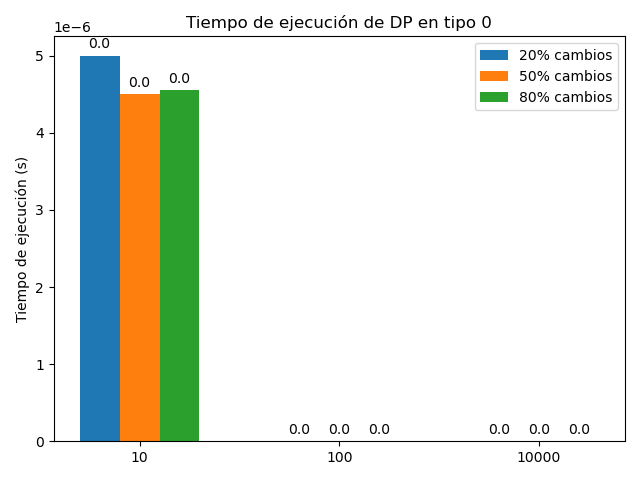
\includegraphics[width=\textwidth]{images/0_bruteforce.png}
    \end{minipage}%
    \begin{minipage}[t]{0.5\textwidth}
        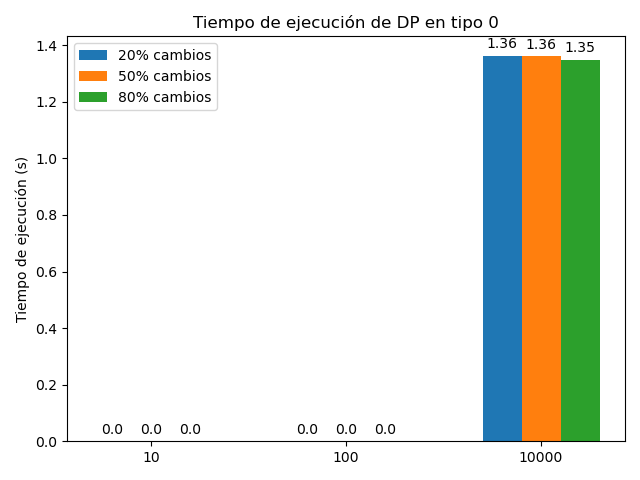
\includegraphics[width=\textwidth]{images/0_dp.png}    \end{minipage}%
    \caption{Tiempo de ejecución de los algoritmos en base a carácteres exclusivamente en mayúscula.}
    \label{fig:scatterplot_3}
\end{figure}

\begin{figure}[H]
    \centering
    \begin{minipage}[t]{0.5\textwidth}
        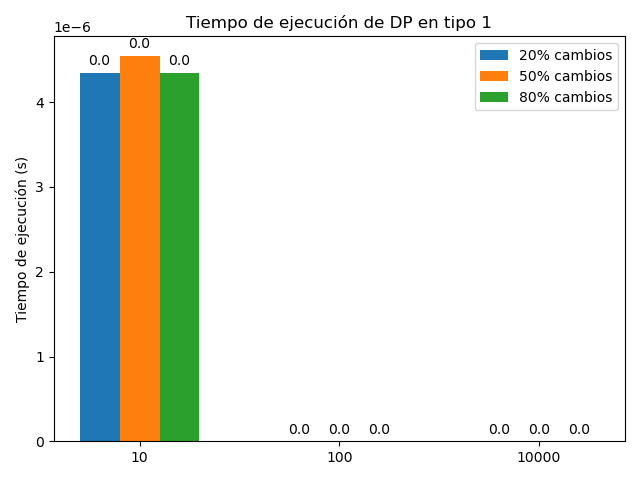
\includegraphics[width=\textwidth]{images/1_bruteforce.png}
    \end{minipage}%
    \begin{minipage}[t]{0.5\textwidth}
        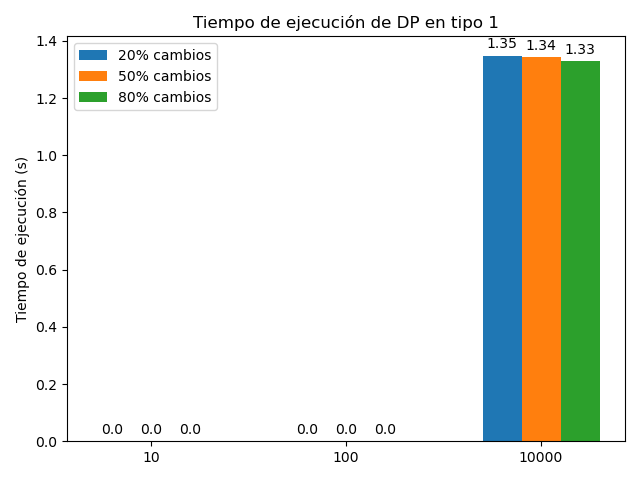
\includegraphics[width=\textwidth]{images/1_dp.png}    \end{minipage}%
    \caption{Tiempo de ejecución de los algoritmos en base a carácteres en mayúscula y en minúscula.}
    \label{fig:scatterplot_3}
\end{figure}

El algoritmo bruteforce sale con tiempo de ejecución 0 para N = 100 y N = 10000. Esto es porque luego de intentar correrlo con un par de strings de tamaño 100, no terminaba de calcular nunca; esto es debido a su complejidad de tiempo antes discutida en el análisis algorítmico (sección 2 del informe). Por tanto, solo se procesaron sus tiempos de ejecución para N = 10.

Notar que incluso para valores chicos de N como 10, el algoritmo de DP ya supera al algoritmo de fuerza bruta, pese a que el primero debe construir la tabla de DP antes de empezar a ejecutar. Esto es tanto un testamento a la rapidez del DP como también la ineficiencia del enfoque de fuerza bruta para este particular algoritmo; si bien no se nota en los gráficos ya que ambos son rondeados a 0.0, examinando las mediciones exactas en las carpetas de measurements, se llega a ver que el algoritmo de DP llega a ser entre 2 y 100 veces más rápido que el de fuerza bruta, particularmente cuando la diferencia entre strings es alta.

Para valores más grandes, como hemos dicho anteriormente, el algoritmo de fuerza bruta no termina de correr nunca. Para N = 100, el algoritmo de DP se ejecuta casi instantaneamente (al punto de quedar nuevamente aproximado a 0.0 en el gráfico), mientras que para N = 10000, se demora poco más de un segundo.

Cabe mencionar que se intentó ejecutar el algoritmo de DP para N = 100000 y N = 1000000, pero no se pudo debido a que la complejidad espacial del algoritmo provoca que se llene la memoria del computador el momento que se intentan procesar pares de string de estos tamaños, aspecto mencionado anteriormente en el análisis del algoritmo. En particular, sólo para N = 100000, la cantidad de memoria requerida para construir la tabla de DP es de (100000*100000*4bytes) = \textbf{37,2 gigabytes} de memoria. Para referencia, mi sistema es de sólo 16GB de RAM, y muchos computadores modernos llegan a tener como mucho 32GB de RAM; algunos sistemas entusiastas tienen 64GB, menos del doble de la cantidad de memoria requerida. Para N = 1000000, ni hablar.


\begin{mdframed}
    Recuerde que es imprescindible que se pueda replicar la generación de las gráficas, por lo que usted debe incluir cómo generó esos datos y  cómo podría generarlos la persona que revisa su entrega y ejecuta sus programas. Por ejemplo, si genera un scatterpolot con Tikz, usted debe explicar cómo obtener la tupla de valores que se usaron para generar la gráfica.
\end{mdframed}


\newpage
\section{Conclusiones}
\begin{mdframed}
    \textbf{La extensión máxima para esta sección es de 1 página.}
\end{mdframed}

Como conclusión, si bien el algoritmo de fuerza bruta sirve para strings chicos, el tiempo de ejecución se dispara totalmente al empezar a trabajar con strings medianos y largos. Se demuestra la superioridad del algoritmo de programación dinámica en este ámbito, sin embargo queda en muestra también su gran debilidad, que es su uso de memoria y la incomputabilidad resultante del algoritmo para strings larguísimos (un caso hipotético de esto siendo la comparación entre dos guiones de película para detectar plagio), por lo que si bien tarda mucho más en llegar a un bloque práctico, este existe.

Al fin y al cabo, no hay algoritmo de oro para un problema; se debe seleccionar el algoritmo a usar en base a las condiciones del input, qué tan rápido se desea el resultado, nuestras limitaciones de memoria, etc.



\newpage

\section{Condiciones de entrega}
% Condiciones generales de tareas de Algoritmos y Complejidad, 20231
  \begin{itemize}
  \item
    La tarea se realizará \tca{individualmente}
    (esto es grupos de una persona),
    sin excepciones.
  \item
    La entrega debe realizarse vía \url{http://aula.usm.cl}
    en un \tca{tarball} en el área designada al efecto,
    en el formato \tca{\texttt{tarea-\tnum-{rol}.tar.gz}}
    (\texttt{rol} con dígito verificador y sin guión).

    Dicho \tca{tarball} debe contener las fuentes en \LaTeXe{}
    (al menos \tca{\texttt{tarea-\tnum.tex}})
    de la parte escrita de su entrega,
    además de un archivo \tca{\texttt{tarea-\tnum.pdf}},
    correspondiente a la compilación de esas fuentes.
  \item Si se utiliza algún código, idea, o contenido extraído de otra fuente, este \textbf{debe} ser citado en el lugar exacto donde se utilice, en lugar de mencionarlo al final del informe. 
  \item
    Asegúrese que todas sus entregas tengan sus datos completos:
    número de la tarea, ramo, semestre, nombre y rol.
    Puede incluirlas como comentarios en sus fuentes \LaTeX{}
    (en \TeX{} comentarios son desde \% hasta el final de la línea)
    o en posibles programas.
    Anótese como autor de los textos.
 
  \item
    Si usa material adicional al discutido en clases,
    detállelo.
    Agregue información suficiente para ubicar ese material
    (en caso de no tratarse de discusiones con compañeros de curso
     u otras personas).
  \item No modifique \texttt{preamble.tex}, \texttt{tarea\_main.tex}, \texttt{condiciones.tex}, estructura de directorios, nombres de archivos, configuración del documento, etc. Sólo agregue texto, imágenes, tablas, código, etc. En el códigos funte de su informe, no agregue paquetes, ni archivos .tex (a excepción de que agregue archivos en \texttt{/tikz}, donde puede agregar archivos .tex con las fuentes de gráficos en \texttt{TikZ}).

\ifprograms
  \item
    Su programa ejecutable debe llamarse \tca{\texttt{tarea\tnum}},
    de haber varias preguntas solicitando programas,
    estos deben llamarse usando el número de la pregunta,
    como \tca{\texttt{tarea\tnum-1}},
    \tca{\texttt{tarea\tnum-2}},
    etc.
    Si hay programas compilados, con en este caso,
    incluya una \tca{\texttt{Makefile}}
    que efectúe las compilaciones correspondientes.

    Los programas se evalúan según que tan claros
    (bien escritos)
    son, si se compilan y ejecutan sin errores o advertencias según corresponda.
    Parte del puntaje es por ejecución correcta con casos de prueba.
    Si el programa no se ciñe a los requerimientos de entrada y salida,
    la nota respectiva es cero.
\fi    
  \item
    %La entrega debe realizarse dentro del plazo indicado en \url{http://aula.usm.cl}:
    La fecha límite de entrega es el día \tca{6 de junio de 2025}.

    \begin{center}
        \Large{
          \textbf{NO SE ACEPTARÁN TAREAS FUERA DE PLAZO}.
        }
        \normalsize
    \end{center}
     
    
  \item
    Nos reservamos el derecho de llamar a interrogación
    sobre algunas de las tareas entregadas.
    En tal caso,
    la nota de la tarea será la obtenida en la interrogación.
    \begin{center}
      \Large{
        \textbf{NO PRESENTARSE A UN LLAMADO A INTERROGACIÓN SIN JUSTIFICACIÓN PREVIA SIGNIFICA AUTOMÁTICAMENTE NOTA 0.}
      }
    \end{center}
    
  \end{itemize}

%%% Local Variables:
%%% mode: latex
%%% ispell-local-dictionary: "spanish"
%%% End:

  
% LocalWords:  tarball tar gz pdf min entregable Makefile puntaje
% LocalWords:  Moodle

\newpage
\appendix


\section{Apéndice 1}
Aquí puede agregar tablas, figuras u otro material que no se incluyó en el cuerpo principal del documento, ya que no constituyen elementos centrales de la tarea. Si desea agregar material adicional que apoye o complemente el análisis realizado, puede hacerlo en esta sección.

\begin{mdframed} 
    Esta sección es solo para material adicional. El contenido aquí no será evaluado directamente, pero puede ser útil si incluye material que será referenciado en el cuerpo del documento. Por lo tanto, asegúrese de que cualquier elemento incluido esté correctamente referenciado y justificado en el informe principal.
 \end{mdframed}


 
\printbibliography

\end{document}


